\documentclass[tikz, border=2pt]{standalone}
% main document, called main.tex
\usepackage{tikz}

\begin{document}

\usetikzlibrary{decorations.pathreplacing}
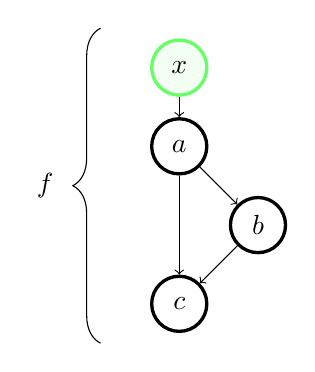
\begin{tikzpicture}[
        scale=1.0,
        inv/.style={circle, draw=green!60, fill=green!5, very thick, minimum size=7mm},
        opv/.style={circle, draw=black, very thick, minimum size=7mm},
      ]
      \node[inv] (x) at (0,3)  {$x$};
      \node[opv] (a) at (0,2)  {$a$};
      \node[opv] (b) at (1,1)  {$b$};
      \node[opv] (c) at (0,0)  {$c$};
      \draw (x) edge[->] (a)
            (a) edge[->] (b)
            (a) edge[->] (c)
            (b) edge[->] (c);

      \draw[
        decorate,decoration={brace,amplitude=10pt}
      ] (-1,-.5) -- (-1,3.5) node[black,midway,xshift=-20pt] {$f$};
    \end{tikzpicture}

\end{document}
